\documentclass[tikz,border=6pt]{standalone}
\usetikzlibrary{arrows.meta,positioning,calc,fit}
\makeatletter
\AtBeginDocument{\global\let\pgf@selectfontorig\relax}
\makeatother

\tikzset{
  state/.style={
    draw=black,
    rounded corners=4pt,
    very thick,
    fill=white,
    minimum width=8.5mm,
    minimum height=7mm,
    align=center,
    inner sep=1.6pt,
    font=\scriptsize
  },
  initial/.style={-Latex, very thick},
  edge/.style={-Latex, thick, shorten >=2pt, shorten <=2pt},
  labelbox/.style={inner sep=3pt, font=\tiny, scale=0.62, transform shape, align=center},
  panel/.style={draw=gray!70, rounded corners=6pt, very thick}
}

\newcommand{\initarrow}[2]{\draw[initial] #1 to (#2);}
\newcommand{\panel}{\draw[panel] (-1.65,-2.65) rectangle (5.85,2.25);}

\begin{document}
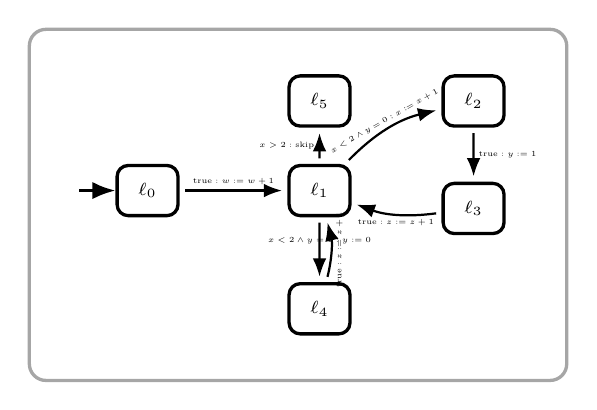
\begin{tikzpicture}[scale=0.91, transform shape]
  \node[state] (p50) at (0,0) {$\ell_0$};
  \node[state] (p51) at (2.4,0) {$\ell_1$};
  \node[state] (p52) at (4.55,1.25) {$\ell_2$};
  \node[state] (p53) at (4.55,-0.25) {$\ell_3$};
  \node[state] (p54) at (2.4,-1.65) {$\ell_4$};
  \node[state] (p55) at (2.4,1.25) {$\ell_5$};
  \initarrow{(-0.95,0)}{p50.west}
  \draw[edge]               (p50) to node[labelbox, above] {$\mathrm{true}:w:=w+1$} (p51);
  \draw[edge, bend left=16] (p51) to node[labelbox, above, sloped] {$x<2\land y=0:x:=x+1$} (p52);
  \draw[edge]               (p52) to node[labelbox, right] {$\mathrm{true}:y:=1$} (p53);
  \draw[edge, bend left=14] (p53) to node[labelbox, below] {$\mathrm{true}:z:=z+1$} (p51);
  \draw[edge]               (p51) to node[labelbox, above] {$x<2\land y=1:y:=0$} (p54);
  \draw[edge, bend right=14](p54) to node[labelbox, below, sloped] {$\mathrm{true}:z:=z+1$} (p51);
  \draw[edge]               (p51) to node[labelbox, left] {$x>2:\mathrm{skip}$} (p55);
  \panel
\end{tikzpicture}
\end{document}
